\newpage
\section{Introduction}
%TODO 细读 1-5 (10th) 节

\subsection{Overview}

\subsubsection{What Operating Systems Do}
操作系统是一个用户与计算机硬件之间的中介程序. 目的: 运行程序, 简化解决问题. 同时重复利用硬件资源. 

\begin{figure}[!htb]
    \centering
    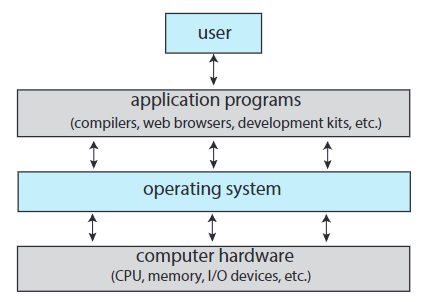
\includegraphics[width=0.309\textwidth]{pic/OS1/Four Components of a Computer System}
    \caption{Four Components of a Computer System}
\end{figure}

\paragraph{Operating System Definition} OS 是资源管理器. 管理资源, 处理冲突以达到资源高效公平的利用. OS 是控制程序. 控制程序运行来防止错误与不适当的电脑使用.

kernel (内核), 始终正在运行的程序. 其他的要么是系统程序(OS提供的)要么是应用程序. 

\paragraph{Computer Startup} 引导程序(bootstrap program)在重启或启动时加载. 其一般存储在 ROM or EPROM (固件, firmware). 

\subsubsection{Computer System Organization}
\begin{figure}[!htb]
    \centering
    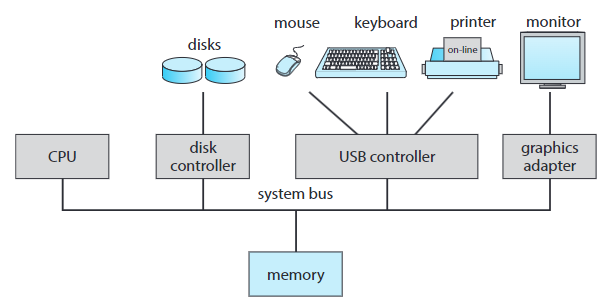
\includegraphics[width=0.42\textwidth]{pic/OS1/A typical PC computer system}
    \caption{A typical PC computer system}
\end{figure}

\paragraph{Computer-System Operation}\quad

\begin{enumerate}%TODO P28-29 补一下
    \item I/O devices and the CPU can execute concurrently. 
    \item 设备通过控制器管理. 
    \item 有 local buffer. IO 通过其与 memory 交换 data. 
    \item CPU 控制 data 的移动
    \item IO 通过
    \item 使用 interrupt 通知
\end{enumerate}


concurrently 与 parallel 都是同时运行但是:
\begin{itemize}
    \item concurrently 非真正同时处理, 但同时开始处理
    \item parallel 同时处理
\end{itemize}

\paragraph{Common Functions of Interrupts}触发 interrupt -> 通过 interrupt vector(存储 routine 起始地址) 查询 -> 运行 interrupt service routine (会保留 context, 通过记录 registers 与 program counter 实现)

interrupt 存在优先级, interrupt 可能会打断 interrupt. 

interrupt 有分类. 例如 software-generated interrupt (又称 trap) 触发来源可能是 error 或者 user request (也称 \textbf{system call}. OS 分为 user code 与 system code, system call 是从 user code 调用 system code). 又例如 hard interrupt. 

OS 是通过 interrupt 驱动的. 好处有: 封装, 管理等. 

在 RISCV 中, interrupt 称为 traps, 分为 interrupt 与 exceptions/ecalls, 分别表示 hard interrupt 与 software interrupt. 

\paragraph{I/O Structure}Two I/O Methods: 在 I/O 开始后,
\begin{enumerate}
    \item (Synchronous 同步, block 阻塞) 等待 I/O 完成后再继续运行 user code 
    \item (Asynchronous 异步, non-block 非阻塞) 不等待 I/O 完成直接继续运行 user code
\end{enumerate}

\begin{figure}[!htb]
    \centering
    \begin{subfigure}{0.22\textwidth}
        \centering
        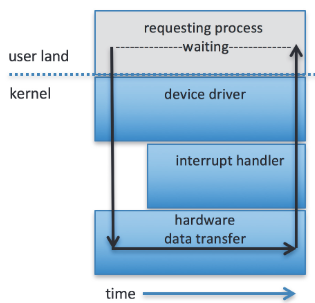
\includegraphics[height=0.9\textwidth]{pic/OS1/Synchronous.png}
        \caption{Synchronous}
    \end{subfigure}
    \begin{subfigure}{0.22\textwidth}
        \centering
        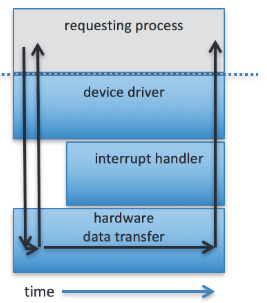
\includegraphics[height=0.9\textwidth]{pic/OS1/Asynchronous.png}
        \caption{Asynchronous}
    \end{subfigure}
    \caption{I/O Methods}
\end{figure}

\begin{figure}[!htb]
    \centering
    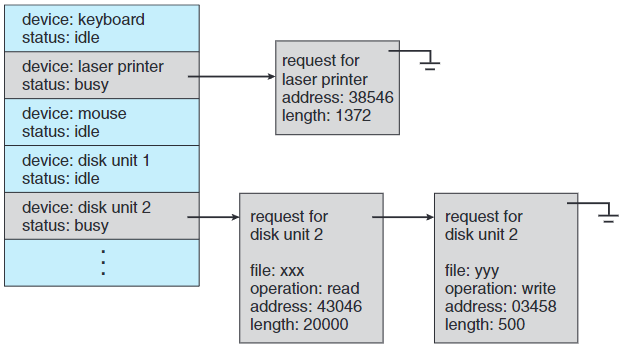
\includegraphics[width=0.309\textwidth]{pic/OS1/Device-Status Table}
    \caption{Device-Status Table (存储设备的状态)}
\end{figure}

\paragraph{Direct Memory Access Structure} CPU 以 block 为单位进行处理 I/O.

\paragraph{Storage Hierarchy} 成本问题, 分层处理, 考虑: 速度, 成本, 变更率. 

\begin{figure}[!htb]
    \centering
    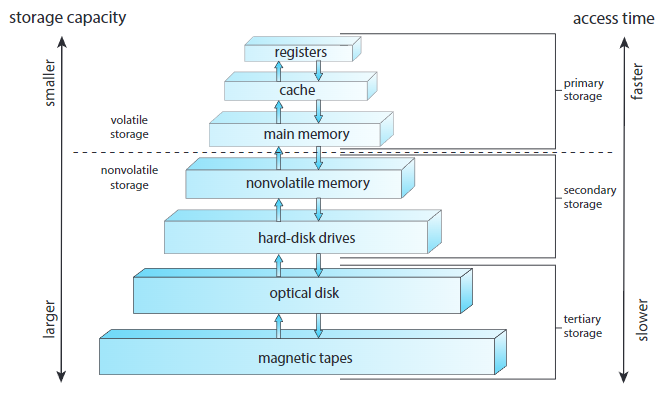
\includegraphics[width=0.42\textwidth]{pic/OS1/storage.png}
    \caption{Storage Hierarchy}
\end{figure}

\paragraph{Caching} 用更高速的设备缓存更低速的设备中的数据的一部分. 

可以解决速度读取速率不匹配的问题. 

\subsubsection{Computer-System Architecture}

\paragraph{Multiprocessor Systems}现在的趋势. 

\begin{figure}[!htb]
    \centering
    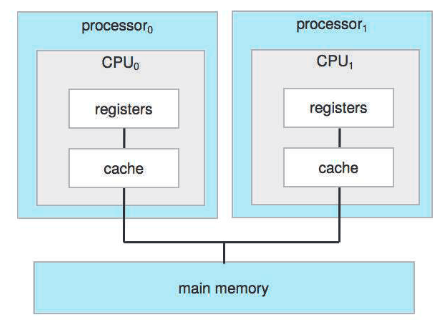
\includegraphics[width=0.309\textwidth]{pic/OS1/Multiprocessor Systems}
    \caption{Multiprocessor Systems}
\end{figure}

\begin{figure}[!htb]
    \centering
    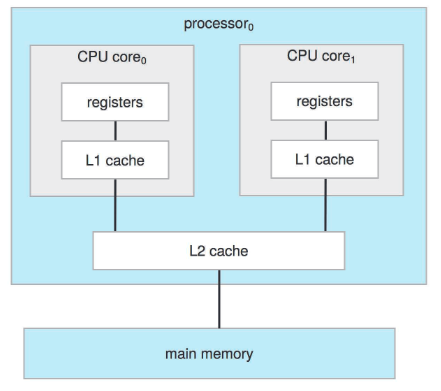
\includegraphics[width=0.24\textwidth]{pic/OS1/Multicore Systems}
    \caption{Multicore Systems}
\end{figure}

\begin{figure}[!htb]
    \centering
    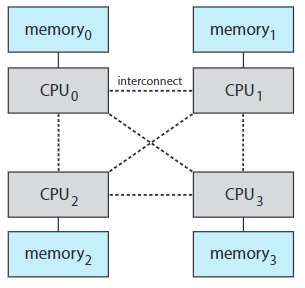
\includegraphics[width=0.24\textwidth]{pic/OS1/NUMA multiprocessing architecture}
    \caption{NUMA multiprocessing architecture}
\end{figure}



\subsection{Structure}
\subsubsection{Operating-System Structure}
\paragraph{Multiprogramming}(多道程序设计) 可在一个 CPU 上运行多个程序, 提高 CPU 利用率. 

\paragraph{Timesharing}(分时系统)(multitasking) 有更好的 interactivity. 计算机可同时服务多个用户, 运行多个任务. 有 swapping 与 virtual memory 机制. 



\subsubsection{Operating-System Operations}
有两个模型: user mode and kernel(supervisor) mode 或可能存在 machine mode. 使用 硬件提供的 mode bit 控制. 

有些 特权 指令只能在 kernel mode 下运行. 

Isolation, 模组之间需要有的隔离. 

\begin{figure}[!htb]
    \centering
    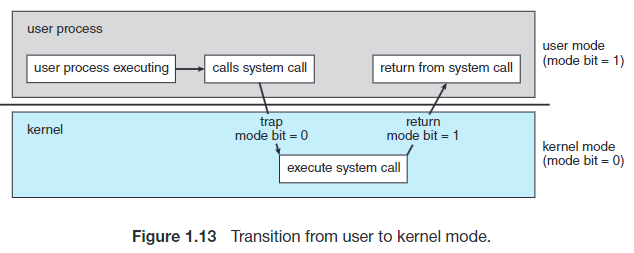
\includegraphics[width=0.42\textwidth]{pic/OS1/Transition from User to Kernel Mode.png}
    \caption{Transition from User to Kernel Mode}
\end{figure}
软中断, trap. 

\subsection{Main parts}
\subsubsection{Process Management}
Program is a passive entity, process is an active entity. 

process(进程) 是资源的集合, 资源有: CPU, memory, I/O, files, initialization data. 进程中止会回收所有资源. 

单线的进程有 program counter (pc), 指明了下一条运行指令的位置. 

多线程的进程每个 thread (线程) 有一个 pc. 

multiplexing (多路复用) the CPUs.

\paragraph*{Activities}:
\begin{itemize}\small
    \item Creating and deleting both user and system processes
    \item Suspending and resuming processes
    \item Providing mechanisms for process synchronization
    \item Providing mechanisms for process communication
    \item Providing mechanisms for deadlock handling    
\end{itemize}

\subsubsection{Memory Management}
所有数据在 processing 之前与之后 需要在 memory 之中. 所有 instructions 需要在 memory 之中. 

\paragraph*{Activities}:
\begin{itemize}\small
    \item Keeping track
    \item Allocating (分配)
    \item data 在 memory 的进出
\end{itemize}

\subsubsection{Storage Management}
磁盘数据最小单位: files. file system 管理文件. 

Mass-Storage Management 海量存储管理. 

\subsubsection{I/O Subsystem}
OS 的目的之一是  hide peculiarities(歧义) of hardware devices. 

I/O subsystem responsible for
\begin{itemize}\small
    \item 高效
    \item I/O 管理统一
    \item 驱动特定的硬件
\end{itemize}


\subsection{OS Purposes}
\begin{itemize}
    \item Abstraction
    \item Multiplex
    \item Isolation
    \item Sharing
    \item Security
    \item Performance
    \item Range of uses
\end{itemize}
